
\title{Recap Computer Architectures (02LSEOV)}
\author{Jacopo Nasi\\
        Computer Engineer\\
        Politecnico di Torino}
\date{I Period - 2017/2018\\\bigskip\bigskip\today}

\documentclass[12pt]{article}
\usepackage[utf8]{inputenc}
\usepackage[italian]{babel}
\usepackage{geometry}
\usepackage{indentfirst} % First line indent
\usepackage{mathtools}
\usepackage{wrapfig}
\usepackage[usenames, dvipsnames]{color}
\usepackage{float}
\usepackage{amssymb}
\usepackage{ifsym}
\usepackage{listings}
\usepackage{multicol}

% Misure Documento
\geometry{ a4paper, total={170mm,257mm},left=35mm, right=35mm, top=35mm, bottom=35mm }

\begin{document}

\begin{figure}
  \centering
  
\includegraphics[width=10cm]{images/polito.pdf}
\end{figure}

\maketitle

\newpage
\tableofcontents

\newpage
{\noindent \Large \textbf{License}\bigskip}

This work is licensed under a Creative Commons Attribution-NonCommercial-ShareAlike 3.0 Unported License.\\
You are free:
\begin{itemize}
  \item \textbf{to Share}: to copy, distribute and transmit the work
  \item \textbf{to Remix}: to adapt the work
\end{itemize}
Under the following conditions:
\begin{itemize}
  \item \textbf{Attribution}: you must attribute the work in the manner specified by the author or licensor (but not in any way that suggests that they endorse you or your use of the work)
  \item \textbf{Noncommercial}: you may not use this work for commercial purposes.
  \item \textbf{Share Alike}: if you alter, transform, or build upon this work, you may distribute the resulting work only under the same or similar license to this one.
\end{itemize}

\noindent More information on the Creative Commons website (http://creativecommons.org).

\begin{figure}[h!]
  \centering
  
\includegraphics[width=3cm]{images/license.png}
\end{figure}

{\noindent \Large \textbf{Acknowledgments}\bigskip}

Questo breve riepilogo non ha alcuno scopo se non quello di agevolare lo studio di me stesso, se vi fosse di aiuto siete liberi di usarlo.\\
Le fonti su cui mi sono basato sono quelle relative al corso offerto (\textbf{Computer Architectures (02LSEOV)}) dal Politecnico di Torino durante l'anno accademico 2017/2018.\\
Non mi assumo nessuna responsabilità in merito ad errori o qualsiasi altra cosa. Fatene buon uso!
\newpage

\section{Introduction Computer Design}
\subsection{Computer Evolution}
The first general-purpose computer was created in the late 40s. What now we can buy for 500\$ is equivalent (performance) to what could be bought for about \$1M in 85'.\\
During the years the performance growth was not linear, as you can see in figure \ref{fig:cpugrowth}, during the first 10 years the annual increase was around 25-30\%/year, from the late 80s to the 2000 the growth is increased around 50\%/year and, in the last few years it decrease to the 22\%. Why this change during the increase?\\
\begin{figure}[h!]
  \centering
  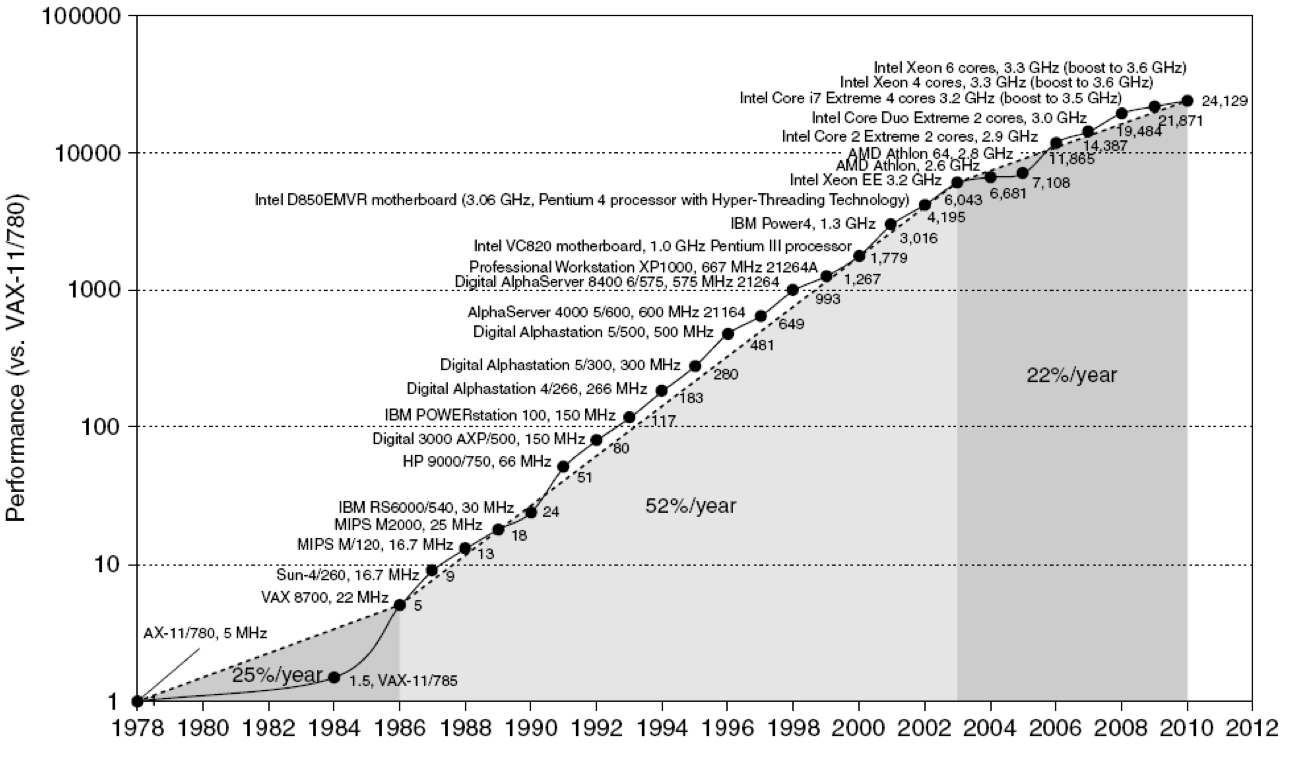
\includegraphics[width=\linewidth]{images/cpugrowth.png}
  \caption{CPUs Growth over years}
  \label{fig:cpugrowth}
\end{figure}
The manufacturers have found a lot of physical problem related to the creation of new products, this problem are mainly related to:
\begin{itemize}
  \item Power-Issue.
  \item Lower instruction-level parallelism.
  \item Unchanged memory lantecy.
\end{itemize}
in fact, since 2004, the major industry have changed the conceptual ways to desing processors, switching from single to multi-core architectures. We can say that, in anytime, this growth is incredible an is due to improvements in technology, microprocessor architecture and software development. Since the multi core introduction the major prefers to investe on multicore system rather than develop faster CPU.\\

\subsection{Designing}
There are 5 main market areas:
\begin{itemize}
  \item \textbf{Personal Mobile Device} (PMD): Smarthphone, tablet. They are focused in energy efficency and real-time app.
  \item \textbf{Desktop Computing}: From PC to workstation and the main pourpose is optimize the price-performance ratio.
  \item \textbf{Server}: Larger-scale and more reliable computing services.
  \item \textbf{Cluster - WAS}:Emphasis on availability, price-performance and power consumption.
  \item \textbf{Embedded Computers}: Fastest growing portion of PCs market. All special-purpose computer-based application, from cheap to high-end processors.
\end{itemize}
There are to \textbf{Classes of Parallelism}:
\begin{itemize}
  \item \textbf{Data-Level} (DLP): Many data items that can be operated on at the same.
  \item \textbf{Task-Level} (TaskLP): Many task of a work can operate independently.
\end{itemize}
The first solution allow the processor to split the data operation over multiple cores, you can for example divide an array of n elements over 4 core and, if T is the computational time needed for the entire array, the final time will be T/4 plus a little time for the reunion of the data. It split the one task on different data.\\
The TLP instead is able to manage multiple task over the same data, this is the common behaviour of the actual system (pipelining techniques).\\
There are different Parallel Architectures:
\begin{itemize}
  \item \textbf{Instruction-level} (ILP): The is modestly use the data-level parallelism.
  \item \textbf{Vector and GPU}: It exploits DLP.
  \item \textbf{Thread-level} (TLP): It exploits DLP and TaskLP.
  \item \textbf{Request-level} (RLP): Exploits parallelism among decoupled (not-related) tasks.
\end{itemize}
The designing of a new computer involve important analysis to the main pourpose of it, you need to study which attributes are important for the new machine and you need to maximizes performance and matching cost and power constraints. During the last decade the PC design took advantage of architectural and technology improvements, the performance increase is more than a factor of 15 on what would have been obtained by relying solely on technology.\\

The \textbf{Moore's Law} says that: \textit{The number of transistors that can be integrated into a single chip doubles every 18/24 months}. Until now the law has worked, as you can see in the figure \ref{fig:moore} and, probably, it will work for other time.

\begin{figure}[h!]
  \centering
  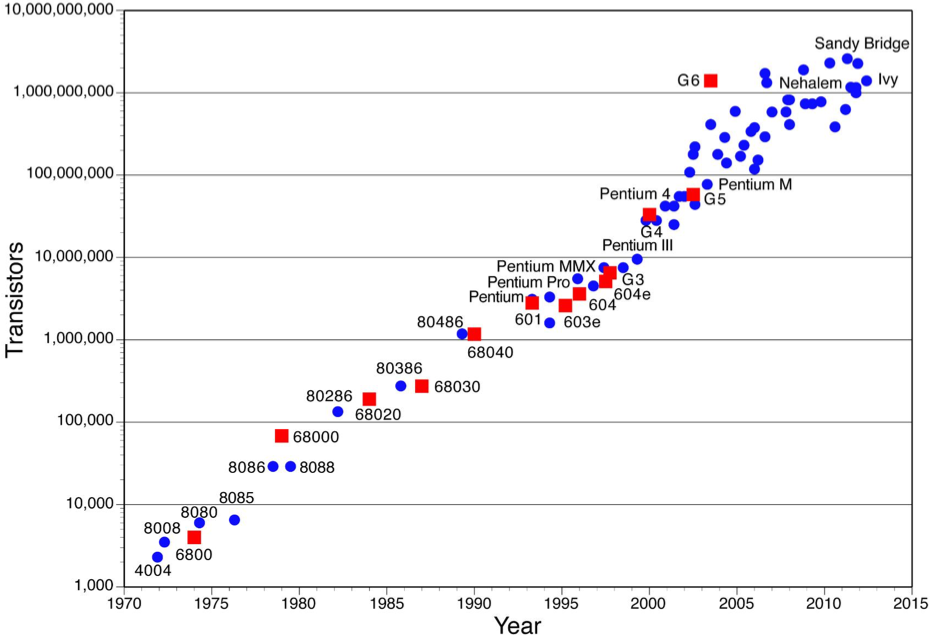
\includegraphics[width=\linewidth]{images/moore.png}
  \caption{Transistors growth on CPUs}
  \label{fig:moore}
\end{figure}

\paragraph{Cost} During the evaluation of the IC manufacturing cost it is important not to forget the impact of yeild, the percentage of products that pass the test phase. The production process for every product undergoes an evolution which normally leads to an improvement in yield (learning curve). The cost decrease is due to yield increase. Probably the most important part of the manufacturing cost is related to the validation and testing procedures.\\

\paragraph{Other designing problem} The continuos increase of the system complexity and device integration leads to porblem with power consumption, for the Power and for the Energy (manly for portable devices). Until now the greater power consumption contribution is due to the trasnsistor switching phase, related to the physical formulas the solution applied is trying to reduce the voltage.\\
Another important factor is the \textbf{Dependability} that is the quality of the system to deliver a correct service, is traditionally very high, but it can be lowered by software or hardware bugs both during the production or in designing phase. During this years the safety-critical areas where the microprocessor have relevant importance are increased, initialy only space, avionics and nuclear, but now we have rail-road, automotive, biomedical, telecom, ecc...\\
The dependability is often measured using:
\begin{itemize}
  \item \textbf{Mean Time To Failure} (MTTF): 1 failure in one billion hours.
  \item \textbf{Mean Time Between Failures} (MTBF)
  \item \textbf{Mean Time To Repair} (MTTR)
\end{itemize}
This three measures are related by the formula: $MTBF = MTTF + MTTR$

\paragraph{Performance} they be analyzed under multiple point of view, \textit{Time between start and completion of an operation, Total amount of work done in time unit, ecc...}. The UNIX system provide 4 different values:
\begin{itemize}
  \item Elapsed time
  \item CPU Time
  \begin{itemize}
    \item User
    \item System
  \end{itemize}
\end{itemize}
The evaluation of often performed letting work a computer and observing its behavior. Unfortunately, the choice of the application severely affects the performance and is not too easy looking the result in a correct way. The main solution is using benchmarks to compare different system running the same operation and production comparable times of execution. The benchmark sets are normally composed of:
\begin{itemize}
  \item Kernels
  \item Program Fragments
  \item Applications
\end{itemize}

There are multiples solution to analyze the performance one of the most common is the \textbf{Amdahl's law} and it based to the comparisons with the older version of the same product. The speedup is calculated by this formula:
\begin{equation}
  \begin{gathered}
    Speedup = \frac{Performance_{enhancement}}{Performance_{NOenhancement}}
    \label{eq:tsoglie}
  \end{gathered}
\end{equation}
the value depends on two factors:
\begin{itemize}
  \item $Fraction_{Enhanced}$: the fraction of the computation time that take advantages of the enhancement.
  \item $Speedup_{Enhanced}$: the suze of the enhancement on the part it affects.
\end{itemize}
A more complete formula is:
\begin{equation}
  \begin{gathered}
    Speedup_{overall} = \frac{1}{(1-Fraction_{Enhanced}) + \frac{Fraction_{Enhanced}}{Speedup_{Enhanced}}}
    \label{eq:tsoglie}
  \end{gathered}
\end{equation}
an example could be useful:\\

\textit{An enhancement makes one machine 10 times faster for 40\% of the programs the machine runs. Which is the overall speedup?}\\
Fraction = 0.4, Speedup = 10.
\begin{equation}
  \begin{gathered}
    Speedup_{overall} = \frac{1}{(1-0.4) + \frac{0.4}{10}} = 1.56
    \label{eq:tsoglie}
  \end{gathered}
\end{equation}

Another important designing evaluation is measuring the time required to execute a program, the are severals approaches:
\begin{itemize}
  \item Observing the real system: Not easy to be evaluated.
  \item Simulation: It could be really expensive.
  \item CPU Equation.
\end{itemize}
the latest solution use a provided formula to evaluate the CPU time:
\begin{equation}
  \begin{gathered}
    CPU_{Time} = CLK_{Time}*\sum_{i=1}^n{CPI_{i}*IC_{i}}
    \label{eq:tsoglie}
  \end{gathered}
\end{equation}
where:
\begin{itemize}
  \item \textbf{$CPI_{i}$}: Number of clock cycles required by instruction i (depends on hardware and instr set).
  \item \textbf{$IC_{i}$}: Number of times instruction i is executed in the program (depends instruction set and compiler).
  \item \textbf{$CLK_{Time}$}: Inverse of clock frequency (depends technology).
\end{itemize}
in the pipelined processor, $CPI_{i}$ may vary for a given instruction, therefore the evaluation becomes much harder.
% END Part 1 - Introduction

\section{Instruction Set Principles}
\subsection{Introduction}
The Instruction Set Architecture (ISA) is hoe the computer is seen by the programmer or the compiler. There are different kind of design and they can be selected by different characteristics. The CPUs are often classified according to the type of their internal storage:
\begin{itemize}
  \item Stack: Is the simplest one it can't accessing memory during operations.
  \item Accumlator: Similar to 8051 can access the memory during operation.
  \item Registers
  \begin{itemize}
    \item Register-memory: Similar to 8086, have a 16-bit register.
    \item Register-Register (load-store)
    \item Memory-memory (no real cases)
  \end{itemize}
\end{itemize}
Nowadays all processors are General-Purpose Register (GPR) this because registers are faster than memoery and are easier for a compiler to use. The CPUs are also classifiable by the number of operant per ALU instruction (2 or 3) and number of memory operand per ALU.\\

\subsection{Memory}
The memory has a fundamental work in the CPU world, there are several different type of it and of course different type to how accessing it.\\
There are many different \textbf{memory addresses} that can be implemented:
\begin{itemize}
  \item \textbf{Little Endian}: Byte with lower address at the least significant position. The addresses of the data is that of the LSB.
  \item \textbf{Big Endian}: Byte with lower address at the most significant position. The addess of the data is that of the MSB.
  \item \textbf{Aligned}: Allowing only aligned accesses to memory could is a limitation in terms of performance.
  \item \textbf{Misaligned}: This solution require hardware and performance overhead.
\end{itemize}
A memory position can be accessed in different ways:
\begin{itemize}
  \item \textbf{Register}: (ADD R4, R3) when a value is in a register.
  \item \textbf{Immediate}: (ADD R4, \#3) for constants.
  \item \textbf{Displacement}: (ADD R4, 100(R1)) accessing local variables.
  \item \textbf{Deferred or Indirect}: (ADD R4, (R1)) accessing using a pointer or a computed address.
  \item \textbf{Indexed}: (ADD R3, (R1 + R2)) useful in array addressing: R1=array base, R2=index.
  \item \textbf{Direct or Absolute}: (ADD R1, (1001)) useful for accessing static data.
  \item \textbf{Indirect}: (ADD R1, @(R3)) if R3 is the addr. of a pointer p, then the mode is like \*p.
  \item \textbf{Autoincrement or decrement}: (ADD R1, (R2)$\pm$) useful for stepping through array within a loop.
\end{itemize}
Is important to choosing the correct addressing mode, one can obtain some important consequences, from reduing the number of instruction to increasing the architecture.\\
There are a lot of instruction that can be done, looking at the 80x86 frequency we can see that most most used are \textit{Load, Conditional Branch, Compare and Store} that are around the 70\% of the total operation performed.\\
The instruction set encoding depends on which instruction compose the instruction set and which addressing modes are supported. When a high number of addressing modes is supported, and address specifier is used to specified the addressing mode. When the number of addressing modes is low, they can be encoded together with the opcode. The different encoding are:
\begin{itemize}
  \item \textbf{Variable}: Any number of operands, operation with variable length, lower performance and minimum code size.
  \item \textbf{Fixed}: Fixed number of operands, need address specifier, fixed instruction length, maximum performance but larger code size.
  \item \textbf{Hybrid}: Multiple format specified by the opcode and it allows a trading-off between code size and performance.
\end{itemize}

Assembly-level programs are now produced by compilers only. The CPU designer and the compiler writer must interact and cooperate. A crucial part taken by the compiler is the optimization of the register using, it easier to solve it when the number of register is higher ($>$16).

\section{Pipelining}
\subsection{Introduction}
Pipelining is an a solution to execute multiple instructions at the same time overlapping it. The different units (also called \textit{stage} or \textit{segment}) are completing different part of different instruction in parallel. The figure \ref{fig:pipe_ex} is an example of this techniques.
\begin{figure}[h!]
  \centering
  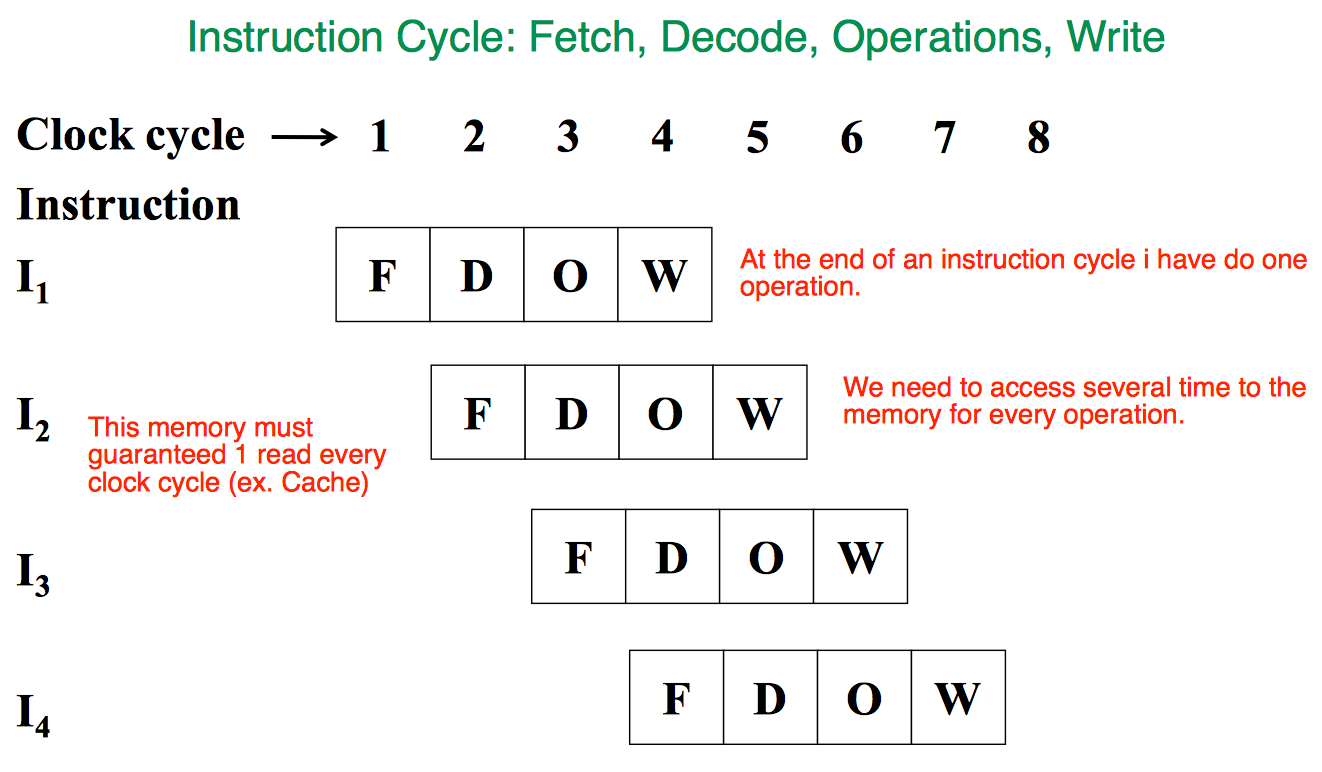
\includegraphics[width=\linewidth]{images/pipe_ex.png}
  \caption{Pipeling example}
  \label{fig:pipe_ex}
\end{figure}
The \textbf{throughput} of a pipelined processor is the number of instructions which exit the pipeline in the time unit. All the pipeline stages are synchronized (they proceed to executing the new task all together); the necessary time for executing one step is called machine cycle and, normally, corresponds to one clock cycle. Of course the duration of a machine cycle is determined by the slowest stage. CPI means clock cycles per instruction. The ideal pipeline have all stages perfectly balanced, in this way the $TRP_{pipelined} = TRP_{unpipelined} * n$ where \textit{n} is the number of pipeline stages.

\subsection{Behaviour}
The execution of each instruction may be composed of at most five clock cycles:
\begin{itemize}
  \item \textbf{IF}: Fetch the instruction from the memory address of the PC and save it in the IR.
  \item \textbf{ID}: Decode the instruction just fetched.
  \item \textbf{EX}: Execute the instruction.
  \item \textbf{MEM}: Memory access and brach completion.
  \item \textbf{WB}: Write-back.
\end{itemize}
with the unpipelined processor all instruction require 5 CC, the only optimization to reduce the average CPI is completing the ALU instruction during the MEM cycle, hardware resources could be optimized avoiding duplications.\\
The pipelined version instead can be more powerful beacause a new instrcution is started at each clock cycle and different  resources work on different instruction at the same time. There are several consideration to keep in mind during the development of this units; at every clock cycle, each resource can be used for one purpose only, this means that:
\begin{itemize}
  \item Separate instruction and data memories must be used.
  \item The register file is used in two stages: for reading (second half of CC) in ID stage and for writing (first half od CC) in WB stage.
  \item The PC (\textit{Program Counter}) must be changed in the IF stage, What about branches?
\end{itemize}
A little view of the system behaviour in figure \ref{fig:time_evo_pipe}.
\begin{figure}[h!]
  \centering
  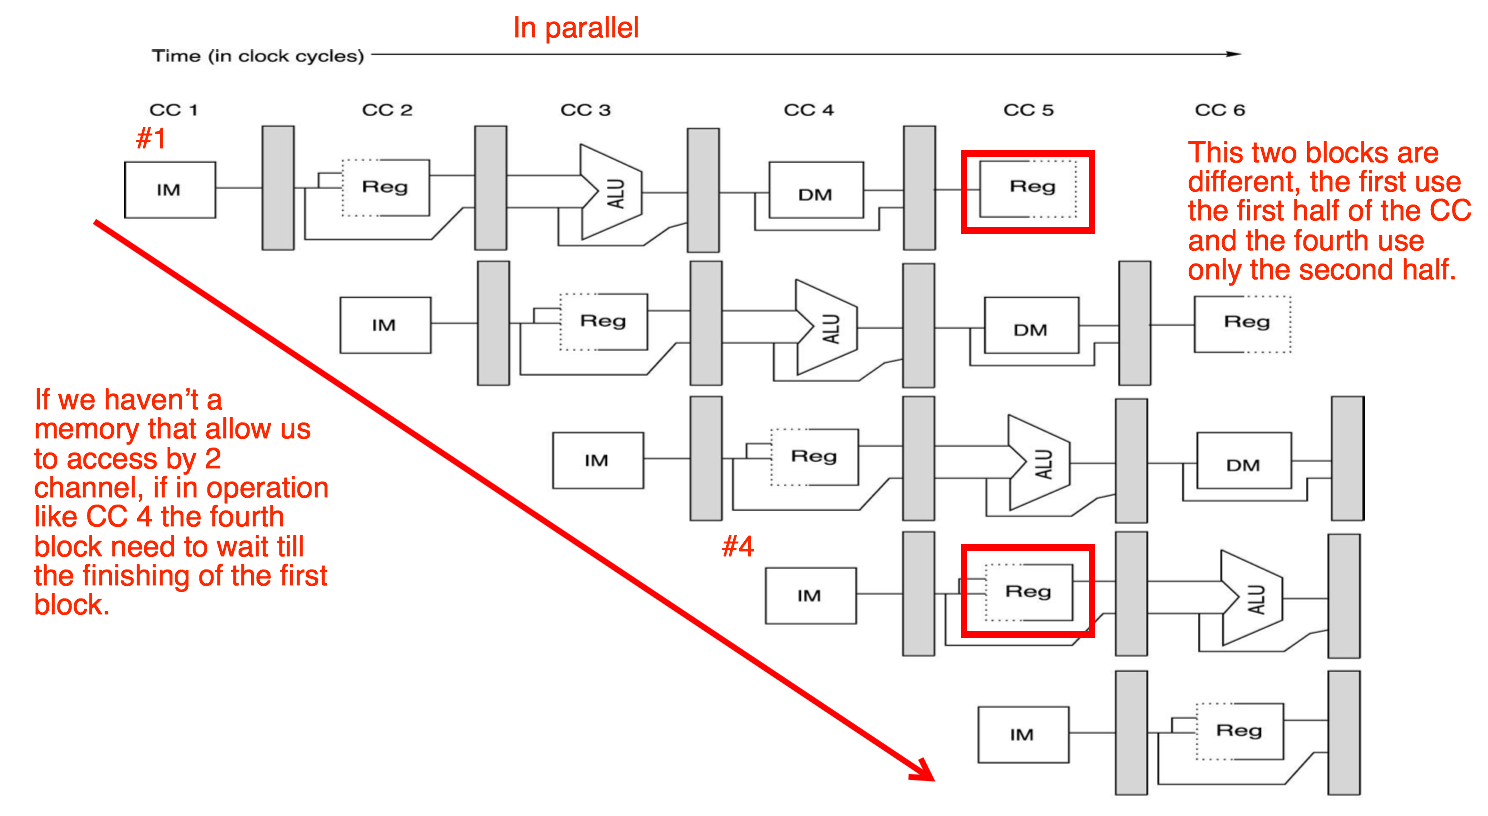
\includegraphics[width=\linewidth]{images/time_evo_pipe.png}
  \caption{Evolution in time of Pipeling architecture}
  \label{fig:time_evo_pipe}
\end{figure}

\paragraph{Performance} The first puorpose of this architectural type is the performance increase without making single instruction faster. The single instruction are maded slower for the overhead introduced by the pipeline control. The limitations of a pipeline come from the necessity of balanced stages and pipeling overhead (pipeline register delay and clock skew).

\subsection{Hazards}
The hazards are situations that prevent the execution of an instruction during its designated clock cycle. There are 3 classes of hazards:
\begin{itemize}
  \item \textbf{Structural}: Coming from resource conflict.
  \item \textbf{Data}: And instruction depends on the result of a previous instruction.
  \item \textbf{Control}:Depend on pipelining branches and other instructions that change the PC.
\end{itemize}
One way to dealing with hazards is to force the pipeline to stall, i.e., to block instructions for one or more clock cycles. When and instruction is stalled:
\begin{itemize}
  \item The instructions following the stalled instruction are also stalled.
  \item The instructions preceding the stalled instruction continue.
\end{itemize}
A stall causes the introduction of a bubble in the pipeline.

\paragraph{Structural hazards} they may happen when some pipeline unit is not able to execute all the operations scheduled for a given cycle. Example:
\begin{itemize}
  \item A given unit is not able to complete its task in one clock cycle (division).
  \item The pipeline owns only one register-file write port, but there are cycles in which two register writes are required.
  \item The pipeline refers to a single-port memory, and there are cycles in which different instructions would like to access to the memory target.
\end{itemize}
Solving this problem implies adding or improving the hardware.

\paragraph{Data hazards} overlapping the execution of instructions, as it is done by pipelining, changes the order of read/write accesses to operands. This can lead to wrong results and undeterministic behaviour.\\
An example could be:\\
\begin{lstlisting}
ADD R1, R2, R3
SUB R4, R1, R5
AND R6, R1, R7
\end{lstlisting}
The second instruction will read the value of R1 before the first instruction can write the new value. This will cause a wrong result. And is the same of course for the third instruction.\\
If an \textbf{Interrupt effects} occurs during the execution of a critical piece of code (from the pov of data hazards) correctness may be restored. This may causa an undeterministic behaviour.\\
There are two possibile solution for data hazards problems:
\begin{itemize}
  \item The first is using the stall till the data will be available.
  \item Implementing the \textbf{forwarding} technique.
\end{itemize}

\paragraph{Forwarding} A special hardware in the datapath detects when a previous ALU operation should write the register corresponding to the source of the current ALU. In this case, the hardware, selects the ALU result as the ALU input rather than the value from the register file. This part must be able to:
\begin{itemize}
  \item Forward a data from any of the previously started instructions (the data can't be already writed in its final location).
  \item Not to forward anything, if the following instruction is stalled, or an interrupt occurred.
\end{itemize}
an example can be viewed in the figure \ref{fig:forward_ex}.

\begin{figure}[h!]
  \centering
  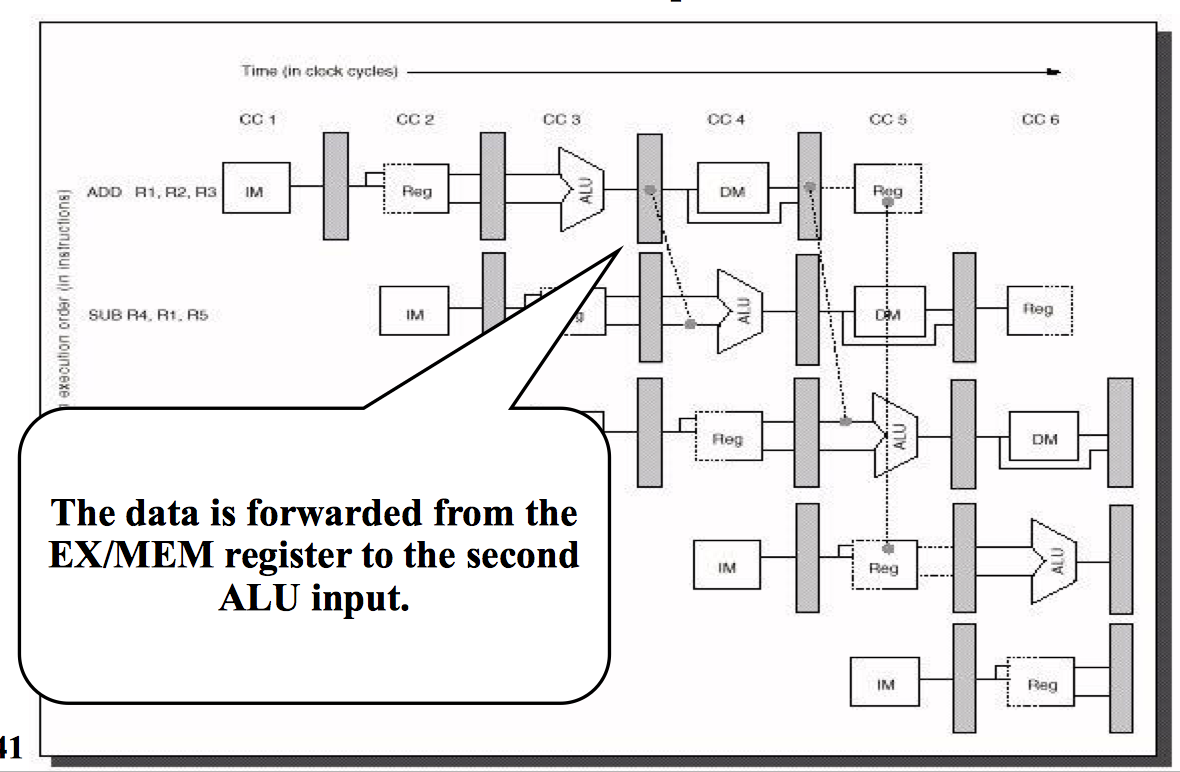
\includegraphics[width=\linewidth]{images/forward_ex.png}
  \caption{Forwarding Example}
  \label{fig:forward_ex}
\end{figure}

The forwarding can be implemented:
\begin{itemize}
  \item From the ALU or data memory output...
  \item ...to ALU inputs, data memory inputs, or the zero detection unit (branch instruction).
\end{itemize}
and the logic must compare:
\begin{itemize}
  \item The DEST fields of the IR in the EX-MEM and MEM-WB register with...
  \item ... the SRC fileds of the IR in the IF-ID, ID-EX and EX-MEM registers.
\end{itemize}

\paragraph{Causes of Data Hazards} A hazards is created whenever there is dependence betweem instructions, and they are close enough that the overlap caused by pipeling would change the order of access to an operand.
In general, this can happen for:
\begin{itemize}
  \item Register Operands
  \item Memory Operands:
  \begin{itemize}
    \item Acceses to memory by load and store are not made in the same stage.
    \item execution can proceed while an instruction waits for a cache miss to be solved.
  \end{itemize}
\end{itemize}
The forwarding not solve all potential data hazards, in this case to only solution is to use stalls.

\paragraph{Stalls} At each clock cycle all test for detecting data hazards are performed (ID stage), if an hazard is detected two actions can be taken:
\begin{itemize}
  \item The apporpriate forwarding is enabled.
  \item The instruction is stalled before entering in the wrong stage.
\end{itemize}
This situation can be performed in two ways:
\begin{itemize}
  \item Forcing all 0s in the ID-EX pipeline register (\textit{nop} instruction).
  \item Forcing the IF-ID pipeline register to maintain the current value.
\end{itemize}

\paragraph{Control Hazards} are due to branches, which may change the PC after the following instruction has been fetched already. In the case of conditional branches, the decision on whether the PC should be modified or not can be taken even later. In the MIPS implementation, the PC is written with the target address (if the jumo is taken) at the end of the ID stage.\\
A possible solution is based on stalling the pipeline as soon as a branch instruction is detected (ID stage) by:
\begin{itemize}
  \item Decide earlier whether the branch has to be taken or not.
  \item Compute earlier the new PC.
\end{itemize}

\paragraph{Performance} there are several techniques for reducing the performance degradation due to branches:
\begin{itemize}
  \item \textbf{Freezing pipeline}: the pipe is stalled until the decision about the branch is know.
  \item \textbf{Predict untaken}: Assume the branch is not taken, avoid any change in the pipe, undo all performed if the branch is taken. *
  \item \textbf{Predict taken}: If the target address is know before the branch outcome, it may be possible to assume the branch as taken. *
  \item \textbf{Delayes branch}: Filling the slot after the branch instruction (branch-delay slot) with instructions which have to be executed no matter the branch outcome. Is a compiler task. Less used nowadays.
\end{itemize}
* This thecniques can be speeded by the compiler which maximizes the chance for the processor to make the right prediction.\\

\subsection{Exception}
The execption are fundamental for system. The are a lot of possible causes:
\begin{multicols}{2}
  \begin{itemize}
    \item I/O device request
    \item System call by user program
    \item Tracing instruction execution (like debug mode)
    \item Breakpoint
    \item Overflow and underflow
    \item FP anomaly
    \item Page fault
    \item Misaligned memoery accesses
    \item Undifined instruction
    \item Hardware malfunction
    \item Power failure
  \end{itemize}
\end{multicols}
they can be calssified based on the type:
\begin{itemize}
  \item \textbf{Synchronous - Asynchronous}: Same position in code - External devices.
  \item \textbf{User requested - Coerced}: Like procedures - Out of user control.
  \item \textbf{User maskable - Non maskable}: Force hardware not to answer to exception requests.
  \item \textbf{Within - Between instructions}: Generated by instruction itself.
  \item \textbf{Resume - Terminate}: Terminate or execute something than resume.
\end{itemize}

There are some machine, called restatable, the are able to handle an exception, save the state, and restart without affecting the execution of the program. Nowadays all processors are restatable.\\

\paragraph{Stopping execution} when and exception occurs, the pipeline must execute the following steps:
\begin{itemize}
  \item Force a trap instruction into the pipeline on the next IF stage.
  \item Until the trap is taken, turn off all writes for the instruction that raised the execption and for all the following instructions in the pipeline.
  \item When the exception-handling procedure receives control, it immediately saves the PC of the faulting instruction.
\end{itemize}
after the exception has been handled, special instructions return the machine from the exception by reloading the PC and restarting the instruction stream.\\
A processor has precise execeptions if the pipeline can be stopped so that:
\begin{itemize}
  \item The instructions just before the faulting instruction are completed.
  \item The instructions following the faulting instruction ca be restarted from scratch.
\end{itemize}
It could be really hard restarting after exception, but precise execption is a must for most architectures, at least for integer.

\paragraph{Contemporary exception} for example we can have 2 different instruction LD that thrown an exeception during the MEM phase and a DADD that can generated an arthmetic exception during the EX phase. The handling could manage the first problem, and if its cause is removed, the second occurs. The situation can be different supposing that the DADD generate an error in the IF stage and the LD still in the MEM phase, this case generate before the DADD exception and then the other.\\
The are multiple solution, a good one could be:
\begin{itemize}
  \item A status flag is associated to each instruction in the pipeline.
  \item If an instruction causes an exception, the status flag is set.
  \item If the status flag is set, the instruction can not perform any write operation.
  \item When an instruction reaches the last stage, and its status flag is set, an exception is triggered.
\end{itemize}
In some cases machines have instructions that change the state before they are committed (those using autoincrement addressing modes). If one of these instructions is aborted because of an exception, it leaves the machine state altered. Implementig precise exceptions could be really tough.\\
Instructions implicitly updating condition codes create complications:
\begin{itemize}
  \item Data Hazards
  \item Save and restored in case of exception.
  \item Hardening the compiler work to filling delay slots between writing conditions and branch.
\end{itemize}

\subsection{Multicycle Operations}
Floating points units perform more complex operations than the integer ones. Forcing them to be executed in a single CLK means using a very slow clock or using really complex unit. The main solution is repeating the EX stage as many times as the instruction requires. An example for undestan the number can be viewed in this table below:

\begin{center}
  \begin{tabular}{ |c||c|c| }
    \hline
    \textbf{Functional Unit} & Latency & Init Interval\\
    \hline
    \textbf{Integer ALU} & 0 & 1\\
    \hline
    \textbf{Data Memory} & 1 & 1\\
    \hline
    \textbf{FP Add} & 3 & 1\\
    \hline
    \textbf{FP/Int Multiply} & 6 & 1\\
    \hline
    \textbf{FP/Int Divide} & 24 & 25\\
    \hline
  \end{tabular}
\end{center}
\textbf{Latency}: It is the number of cycles that should last between an instruction that produces a result and an instruction that uses the same result.\\
\textbf{Initiation Interval}: It is the number of cycles that must elapse between issuing two operations of the same type to the same unit.\\

\paragraph{Hazards} can be more frequent due to the different structure of the EX stage. This because:
\begin{itemize}
  \item Unpipelined divide unit, where several instructions could need it at the same time.
  \item The instructions have varying running times, the number of the register writes required in a cycle can be larger that 1.
\end{itemize}
solving this problem with more writes ports is normally too expensive, the solution is forcing a structural hazard stalling the instructions in the ID stage, or stalling it before the MEM or WB stage. This kind of operations can introduce long period of stall. This introduce new type of hazards, like \textbf{RAW} (Read After Write), \textbf{WAW} (Write After Write) and  structural hazards involving the divide unit and the write port.\\
A solution could be that, before issuing an instruction to the EX phase, check whether it is going to write on the same register of an instruction still in the EX stage. In this case, stall the new instruction. Of course guarantee the precise exception become really hard, the possible solutions are:
\begin{itemize}
  \item Accepting imprecise execeptions.
  \item Fast, but imprecise operating mode, and slow, but precise one.
  \item Buffering the results of each instruction until all the previously issued instructions have been completed.
  \item Forcing the FP units to early determine whether an instruction can cause an exception, and issuing further instructions only when the previous ones are guaranteed not to cause an exception.
\end{itemize}
An alternative solution is like the MIPS R4000 that implements a 8 cycle pipelined processors. This means more forwarding, increased load delay slot and increased branch delay slot.

\section{Instruction Level Parallelism}
The pipelines exploit the parallelism existing among instructions, which allows their execution in parallel. The highest the amount of ILP that can be found, the better the performance of the pipeline. There are two kind of approach:
\begin{itemize}
  \item Static: Depending on the software (i.e compiler). Used in embedded system.
  \item Dynamic: depending on the hardware to locate parallelism. Used in desktop and server.
\end{itemize}

The basic block is the group of instructions belonging to the same block, it means no branches in (except entry) and no branches out (excepts exit). The basic block is opmizable by the compiler by a little rescheduling. For example if we need to compute $a=b+c\\d+e-f$ on solution could be the one in figure \ref{fig:stall}:
\begin{figure}[h!]
  \centering
  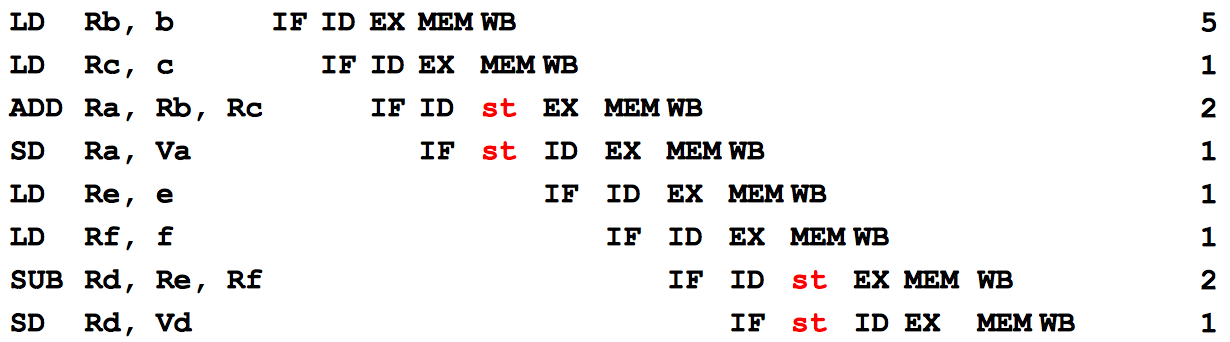
\includegraphics[width=\linewidth]{images/stall.png}
  \caption{First execution order}
  \label{fig:stall}
\end{figure}
that requires 14 clocks cycles. In figure \ref{fig:stall2} a better solution is implemented, this rescheduling requires only 12 clock cycles.
\begin{figure}[h!]
  \centering
  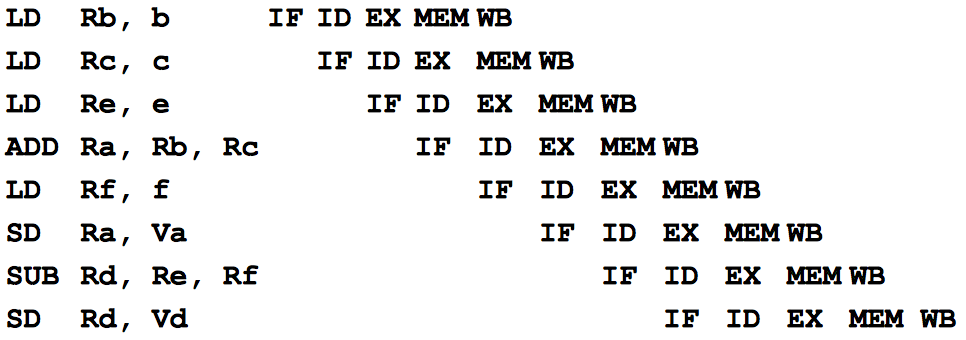
\includegraphics[width=\linewidth]{images/stall2.png}
  \caption{Second execution order}
  \label{fig:stall2}
\end{figure}
 For typical MIPS program the size of a basic block is between 4 and 7 instructions. Since these instructions are likely to be dependent one from the other, the amount of parallelism existing within a basic block is normally rather small.\\
 COnsidering a loop any iteration of a loop could be independent on the others, so they can be overlapped. There are two ways for exploting the loop-level parallelism:
 \begin{itemize}
   \item Loop unrolling (static or dinamyc)
   \item SIMD
 \end{itemize}

The first solution explicitly replicate the loop body in multiple times like in figure \ref{fig:unrolling}.
\begin{figure}[h!]
  \centering
  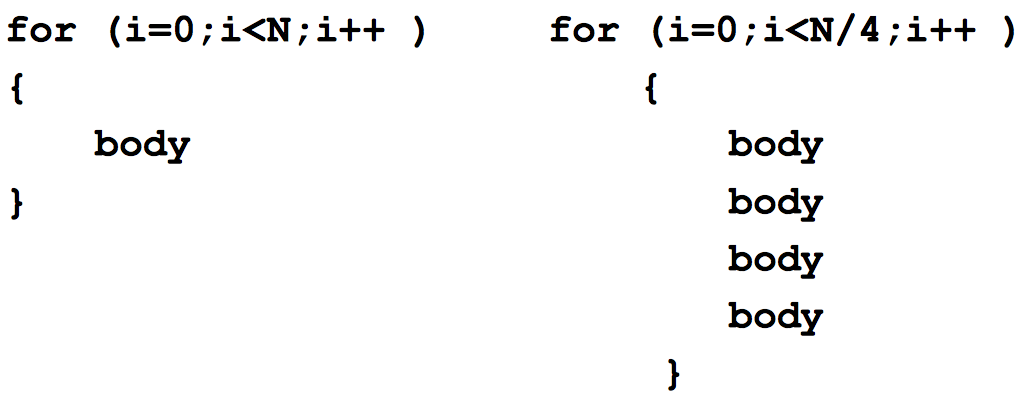
\includegraphics[width=\linewidth]{images/unrolling.png}
  \caption{Loop unrolling}
  \label{fig:unrolling}
\end{figure}
The considerations are:
\begin{itemize}
  \item[\textbf{+}] Reduced overhead due to the iteration control.
  \item[\textbf{+}] Wider body increase the chance for the compiler to exploit rescheduling to eliminate stalls.
  \item[\textbf{-}] Size code increased.
\end{itemize}

The SIMD techniques it can be exploited in:
\begin{itemize}
  \item Vector processors: A vector instruction operates on a set of data, instead of on a scalar data (as normal instructions).
  \item GPUs: Parallel acting over multiple data.
\end{itemize}

In both cases is necessary to evaluate the dependencies, if two instructions are not dependent, they can be executes in parallel without any stall. If they are not, they have yo be executed in order (or partly overlapped). There are 3 kind of dependencies: data, name and control.\\
An instruction \textit{i} is \textbf{DATA} dependent on instruction \textit{j}, if \textit{i} produces a result that is used by instruction \textit{j}, or if j is dependent on instruction \textit{k}, and \textit{k} is dependent on instruction \textit{i}.\\
Detecting dependencies involving registers is easy. Detecting dependencies involving memory cells is much more difficult, because accesses to the same cell can look very different. Using a static techniques force the compiler to adopt a conservative approch, assuming that anu load instruction refers to the same cell of the previous store. This kind of dependencies can be only detected at the tun time, when the addresses are known.\\
A \textbf{NAME} dependencies occurs when two instructions refer to the same register or memory location (name) but there is no flow of data associated to the name. They can be of 2 types:
\begin{itemize}
  \item \textit{Antidependence}: Instruction j writes a register or memory location that instruction i reads, and instruction i is executed first.
  \item \textit{Output dependence}: Both instruction i and j write the same register or memory location.
\end{itemize}
The name dependencies do not prevent from reordering involved instructions, provided that we change the register used by one of the two instructions, it can be exploited by compiler (statically) or by the processor (dynamically). A similar method can be implemented to solve name dependencies involving memory locations.

\end{document}
